\section{Evaluation}
\label{Eva}

\subsection{Evaluation Setup} In this section, we evaluate the performance of {\sdn}
by real-scene experiments. We deploy 100 TI
SensorTag sensors randomly in a $250~\times~250$ square meters area. 
The operating system of sensors is contiki-ng~\cite{}. We use different metrics for various
applications and compare our works with other state-of-the-art works such as RPL
and LEACH. Although Alder implements a sensor system using UAVs, it doesn't
provide a complex routing protocol, and thus we do not compare with it on
throughput or latency.

When measuring the network, we make nodes send packets every 10 seconds, and the
packet size is 60 bytes. Unless otherwise specified, we set the evaluation time
from 0 to 8000 seconds.

\subsection{Evaluation Metrics}

\textbf{Packet received ratio} is defined as the proportion of the total data
packets received by data center and the total data packets sent by all nodes, 
we adopt the model in \cite{chen2017energy}
and it can be formulated as
\begin{equation}
	L = \frac{\sum_{i = 0}^{N}S_i}{R}
\end{equation}
where $L$ represents the throughput, and $S_i$ and $R$ denotes the number of
packets sent by the $i$-th node and the number of packets received by data
center, respectively.

\textbf{Throughput} is defined as the the total data packets received by data
center in 10 seconds, and it measures the capability and scalability of a network. 

\textbf{Latency} is defined as the time interval between node sent data package and
data center received the package.

\textbf{Network Lifetime} is defined as the elapsed time when total package
received ratio is less than 50\%, which is an important metric to measure the
reliability of network.

\textbf{Energy Consumption} is estimated by multiplying different coefficients on
CPU running time and radio listening and transmitting time and summing them up.
The coefficients are proportional to the working current described in sensor's
data sheet. Average energy consumption is the energy consumption of a node in
unit time.

\subsection{Basic Routing}

In order to fairly compare with existing works, we first use our basic
{\sdn} routing protocol without any intelligent approaches. We evaluate routing
performance by throughput, packet received ratio and end-to-end latency.
Meanwhile, We also evaluate the scalability of our network through network
lifetime. We do not compare {\sdn} with Alder on throughput and latency because
Alder doesn't implement a complete routing protocol.

%\begin{figure}[htbp]
\begin{figure}[!h]
	\centering
	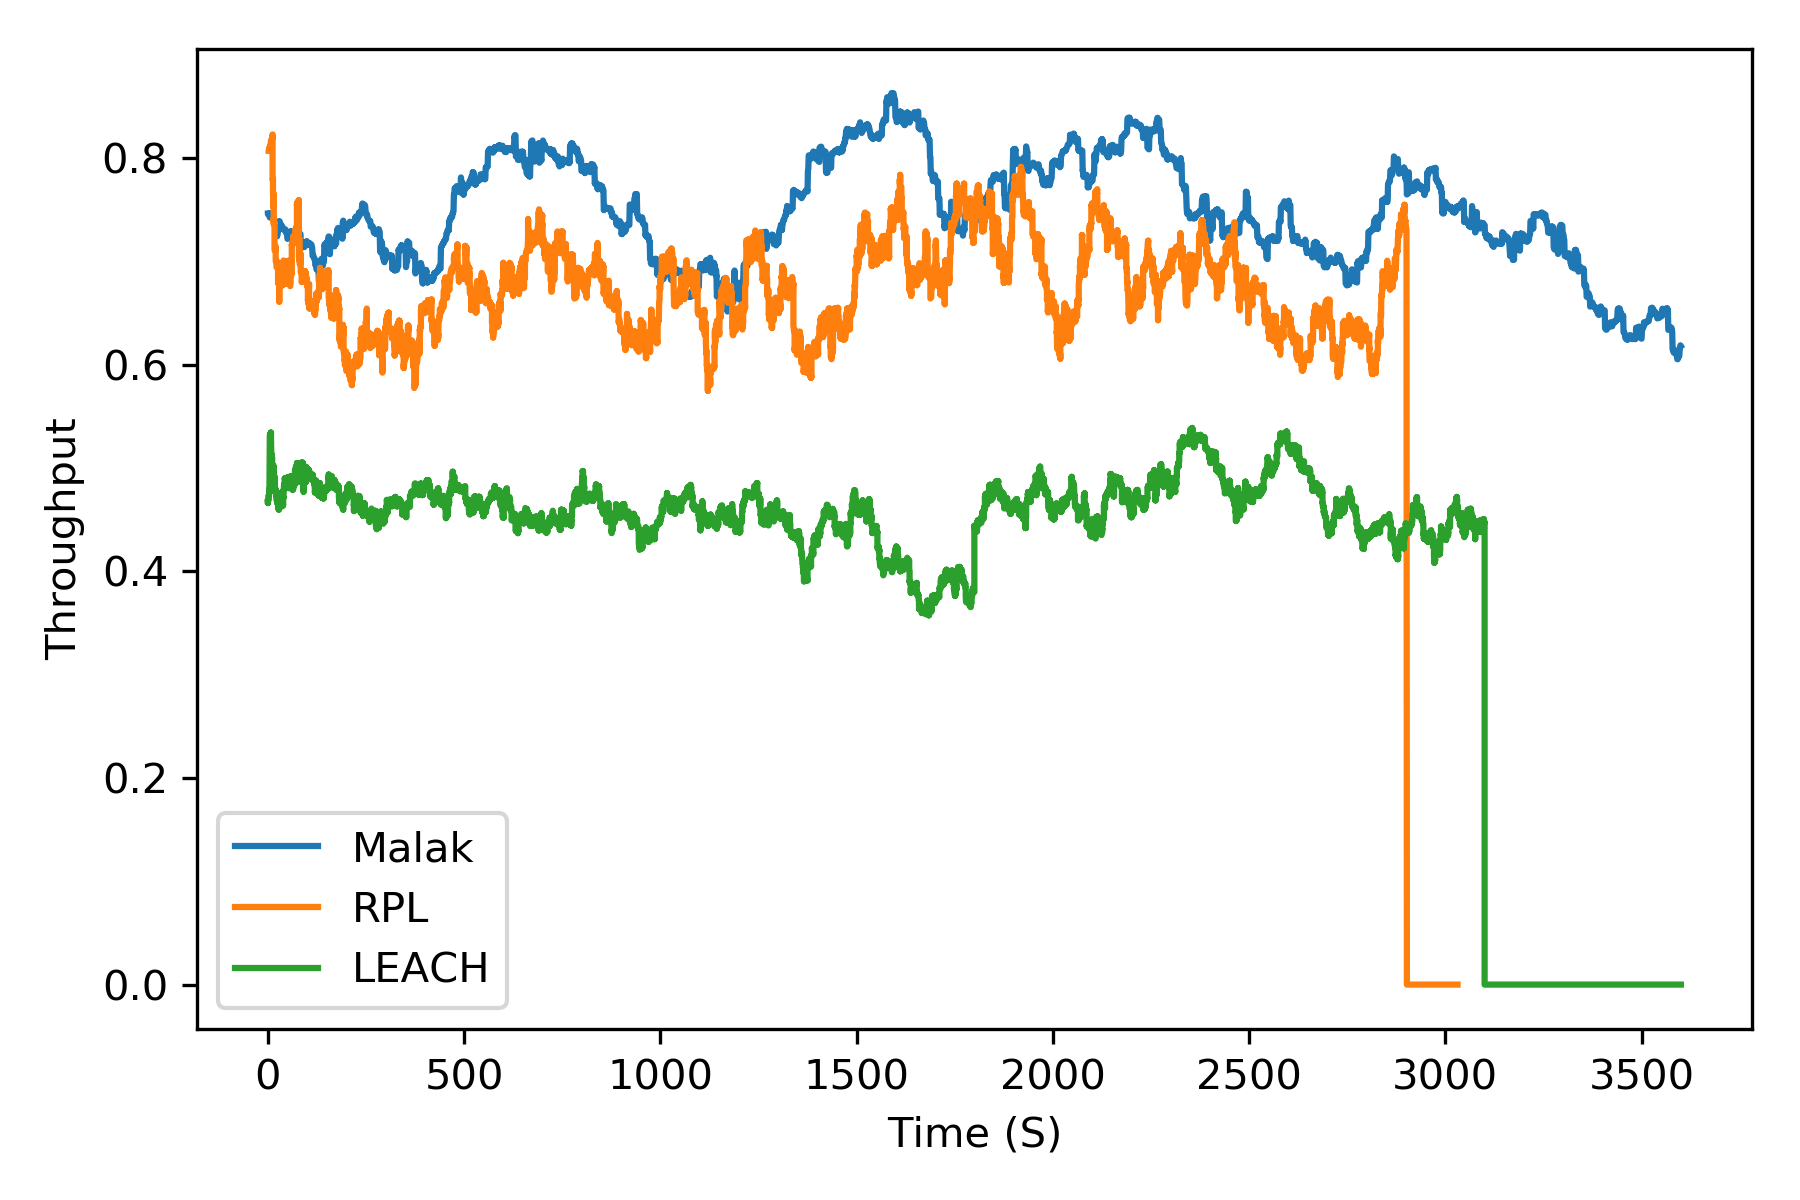
\includegraphics[width=.95\columnwidth]{Figure/throughput}
	\vspace{-0.1in}
	\caption{End-to-end routing throughput.
		\textnormal{
			The {\sdn}'s average of the throughput is 1.7 and 3 times higher within 0
			to 8000 seconds compared with RPL and LEACH, respectively.
	}}
	\label{fig:throughput}
\end{figure}

Figure~\ref{fig:throughput} compares network throughput by deploying various
routing algorithms. As {\sdn} uses OSPF to calculate the route table, which
finds the optimal path from sensors to data center, its throughput exceeds RPL
and LEACH. This implies there are less collisions in {\sdn}. Besides, in {\sdn},
sensors' average lifetime increases by {\totalLife} compared with RPL, since all
compute-intensive tasks are done by UAVs and sensors do not need to send
packets to negotiate route path, which decreases the energy consumption with no
doubt.

%\begin{figure}[htbp]
\begin{figure}[!h]
	\centering
	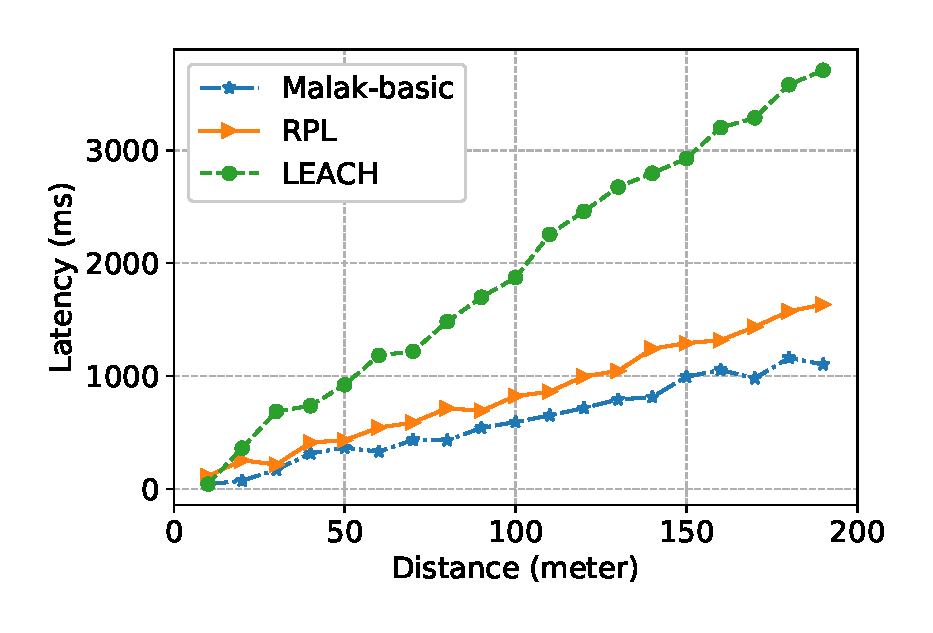
\includegraphics[width=.95\columnwidth]{Figure/latency}
	\vspace{-0.1in}
	\caption{End-to-end average latency of different routing algorithms and distance.
		\textnormal{
	}}
	\label{fig:latency}
\end{figure}

When measuring the latency of the network, the {\sdn} routing method performs
better than RPL due to the use of the global topology information to find the
optimal route path. As shown in Figure~\ref{fig:latency}, as the distance from
node to data center increases, the latency grows about 4 times and 1.5 times
slower than LEACH and RPL, respectively.

%\begin{figure}[htbp]
\begin{figure}[!h]
	\centering
	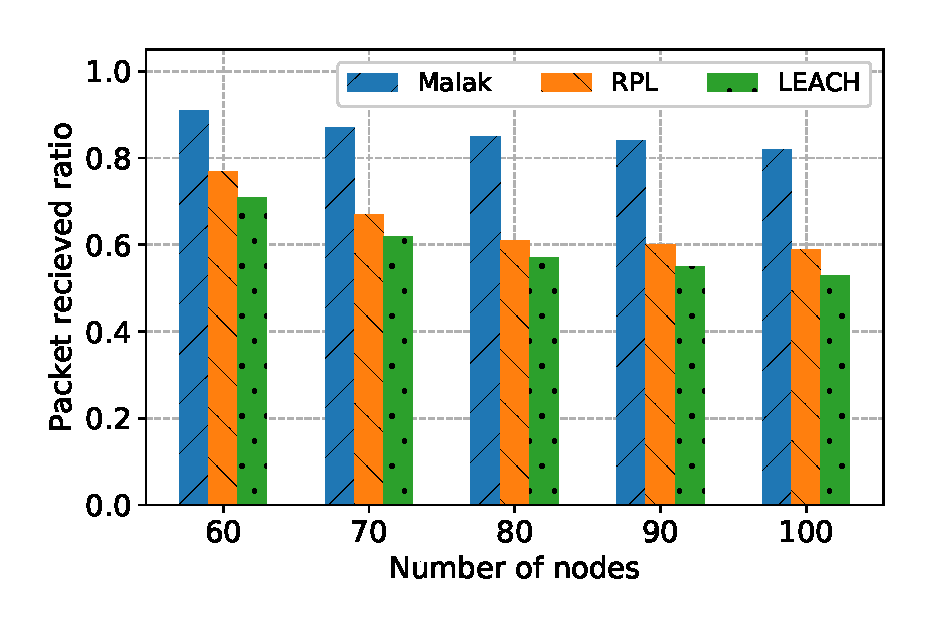
\includegraphics[width=.95\columnwidth]{Figure/packet_loss_ratio_with_size}
	\vspace{-0.1in}
	\caption{Per-node packet received ratio improved by {\sdn}.
		\textnormal{
			This figure shows the {\sdn} reduce collisions of nodes by
			reducing the routing negotiation, and decreases the radio
			transmission.
	}}
	\label{fig:packet_loss_ratio_with_size}
\end{figure}

Figure~\ref{fig:packet_loss_ratio_with_size} shows two remarkable advantages of
{\sdn}: (1) The packet received ratio exceeds state-of-the-art algorithms
RPL\cite{winter2012rpl} and LEACH\cite{kaur2016wsn} by 20\%; (2) With the
increasing of network size, the {\sdn}'s packet received ratio is still 20.2\%
and 28.8\% higher than RPL and LEACH, respectively. There are two reasons: (1) {\sdn}
uses global information to achieve optimal routing, and (2) intelligent cluster
header selection balances the energy consumption between nodes.

%\begin{figure}[htbp]
\begin{figure}[!h]
	\centering
	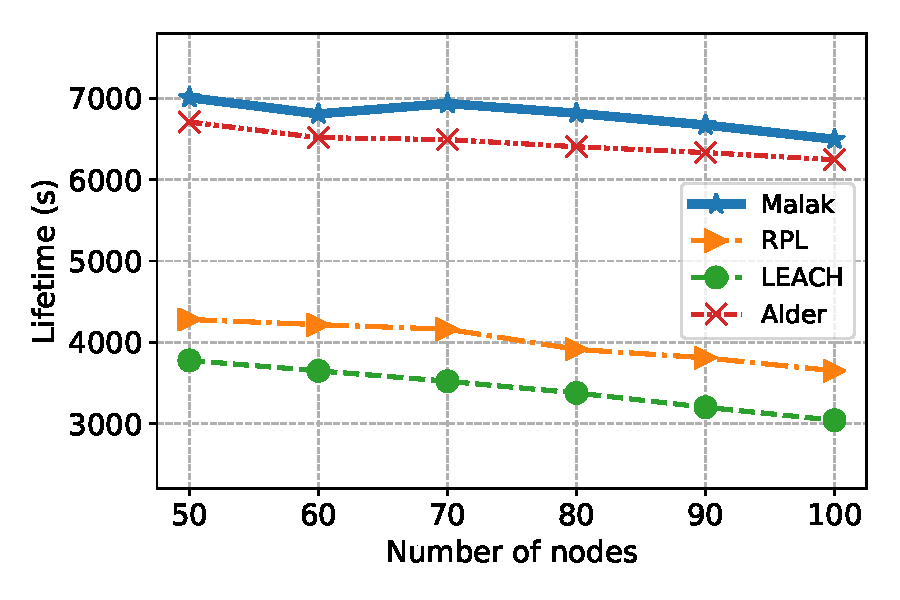
\includegraphics[width=.95\columnwidth]{Figure/lifetime}
	\vspace{-0.1in}
	\caption{Network lifetime using various routing algorithm
		\textnormal{
			{\sdn} surpasses RPL and LEACH in different network sizes.
		}}
	\label{fig:lifetime}
\end{figure}

The{\sdn} system is capable in large scale WSNs as
Figure~\ref{fig:lifetime} shows. Its lifetime excels RPL and LEACH in both
small and large network sizes.

\subsection{AI Applications}

By deploying intelligent node selection algorithm, we use minimum active sensors
to collect necessary sensing data.
%covering the whole area and reduce the redundant ones in the meantime.
Besides, less sensors means less collision and
interference, and it can further improves the reliability of network. And the
packet received ratio grows by 10\%$\sim$15\% and achieves almost 100\% as
Figure~\ref{fig:ai_selection} shows.

%\begin{figure}[htbp]
\begin{figure}[!h]
	\centering
	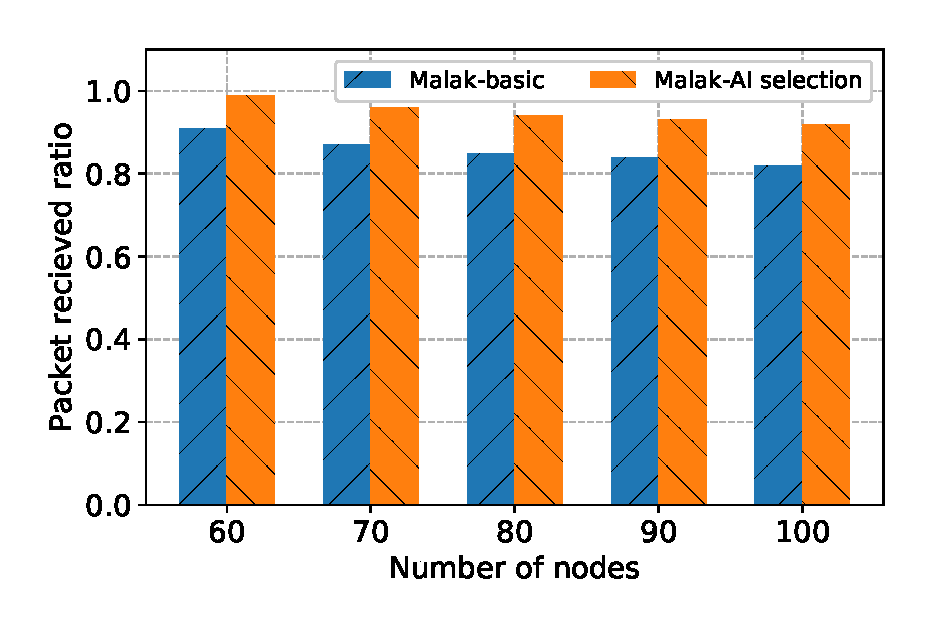
\includegraphics[width=.95\columnwidth]{Figure/ai_selection}
	\vspace{-0.1in}
	\caption{Packet received ratio improved by intelligent node selection
		\textnormal{
		}}
	\label{fig:ai_selection}
\end{figure}

By deploying MLP on UAVs, {\sdn} can predicts the energy consumption precisely as
Figure~\ref{fig:energy_pred} shows, and the absolute error can be restricted in
$0.1$, which enable us to predict and fix energy failure in advance.

%\begin{figure}[htbp]
\begin{figure}[!h]
	\centering
	\hspace{-0.3cm}
	\subfloat[Energy prediction]{
		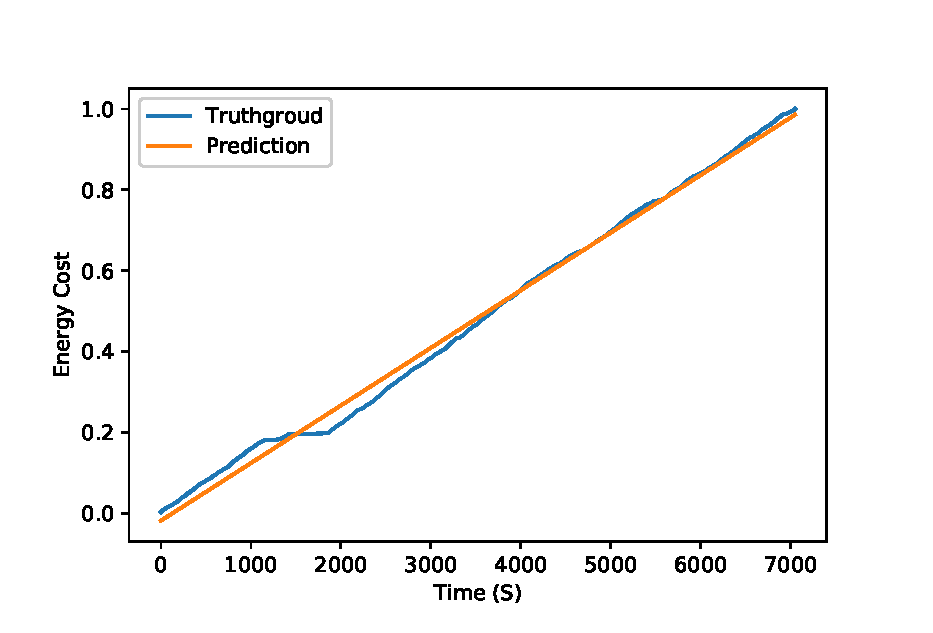
\includegraphics[width=.48\columnwidth]{Figure/energy_pred}
		\label{fig:energy_pred:a}
	}
	\hspace{-0.2cm}
	\subfloat[Prediction error]{
		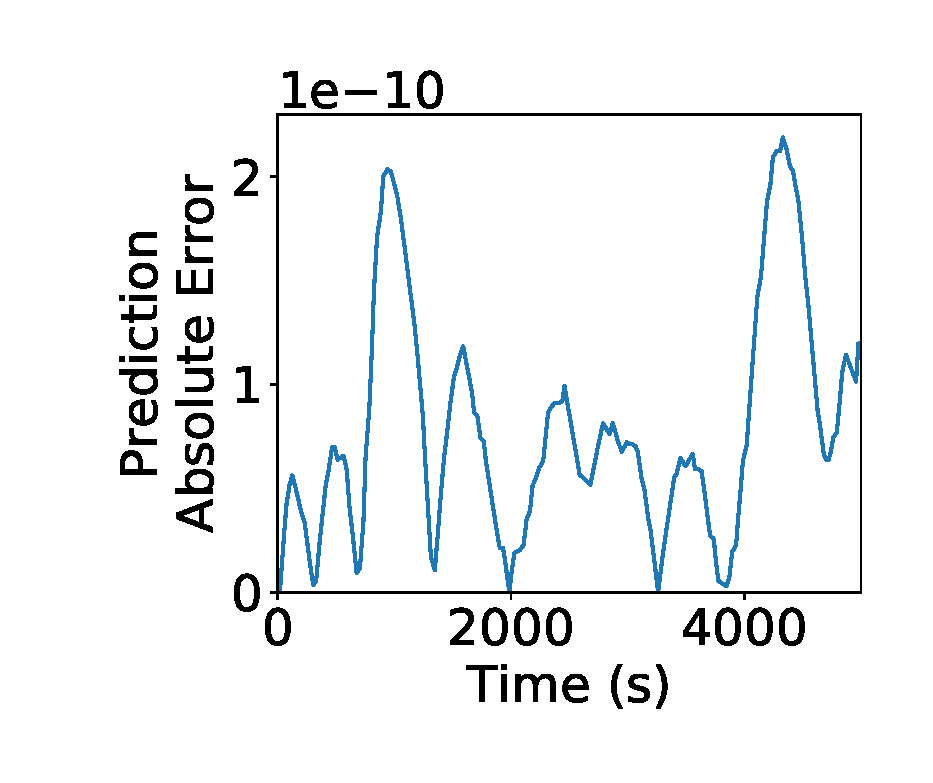
\includegraphics[width=.48\columnwidth]{Figure/energy_pred_err}
		\label{fig:energy_pred:b}
	}
	\vspace{-0.1in}
	\caption{Energy prediction
		\textnormal{
			We use MLP to predict energy consumption and the
			prediction result is consistent with the truth-ground.  The absolute
			error of energy prediction never exceeds $0.1$ with normalized energy
			(i.e. the maximum energy of a sensor is 1).
		}
	}
	\label{fig:energy_pred}
\end{figure}

\subsection{Resilience}

%\begin{figure}[htbp]
\begin{figure}[!h]
	\centering
	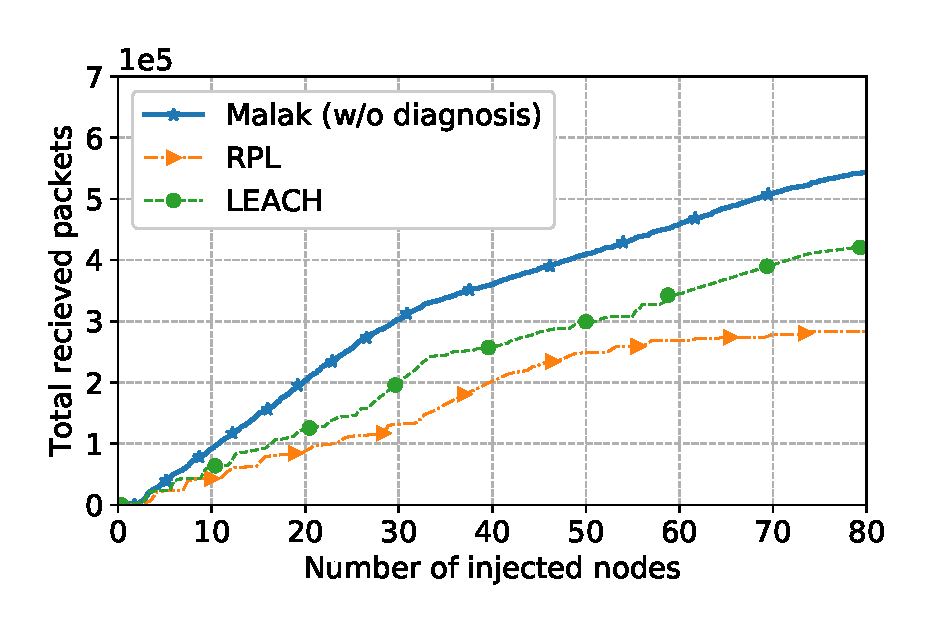
\includegraphics[width=.95\columnwidth]{Figure/fault_tolerance}
	\vspace{-0.1in}
	\caption{Fault tolerance
		\textnormal{
			RPL and {\sdn} are compared on resilience, and {\sdn} perform
			slightly better than RPL.
		}}
	\label{fig:fault_tolerance}
\end{figure}

We compare the impact caused by death of nodes using throughput among LEACH, RPL
and {\sdn} and the results are shown in Figure~\ref{fig:fault_tolerance}. The
total received packets of {\sdn} increases stably due to its resilience to faults
of nodes. The resilience is achieved by 2 approaches: (1) cluster based protocol
is immune from failures of cluster members; (2) Local repair enable the network
recover from failures of cluster headers.

%\begin{table}[htbp]
%	\centering
%	\caption{Failure detection rate for various failure type and number}
%	\label{tab:diagnosis}
%	\begin{tabular}{|c||c|c|c|c|c|}
%		\hline
%		\diagbox{Type}{Failures} & 1 & 2 & 3 & 4 & 5\\
%		\hline
%		\hline
%		Sensing & 98\% & 95\% & 93\% & 92\% & 90\%\\
%		\hline
%		Energy & 100\% & 93\% & 92\% & 90\% & 88\%\\
%		\hline
%		Radio & 100\% & 90\% & 88\% & 84\% & 80\%\\
%		\hline
%	\end{tabular}
%\end{table}

%\begin{figure}[htbp]
\begin{figure}[!h]
	\centering
	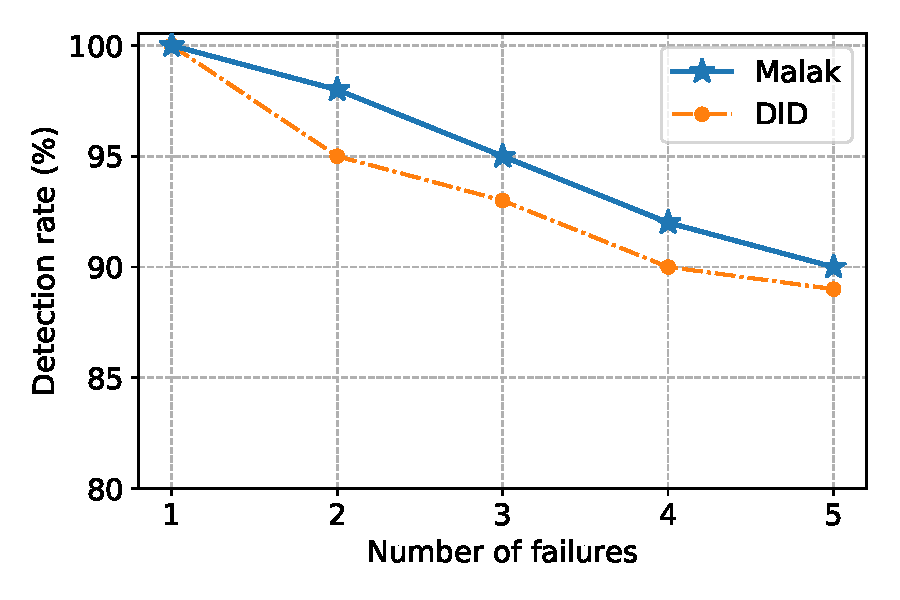
\includegraphics[width=.95\columnwidth]{Figure/did_comp_curve}
	\vspace{-0.1in}
	\caption{Comparation of {\sdn} and DID on failure detection rate.
		\textnormal{
			{\sdn} surpasses DID by using UAVs to lessen dectecting area.
		}}
	\label{fig:did_comp}
\end{figure}

%Table~\ref{tab:diagnosis} shows the failure detection rate among sensing,
%energy and radio failures.
We compare our algorithm with DID\cite{gong2015directional}, but as it is not
open-source, we implement DID by closely following the algorithm proposed in
\cite{gong2015directional} and evaluate it in our settings. The main reason
{\sdn} performs better than DID is that our UAVs can fly to a the fault area
which decrease the number of potential candidate of injected nodes. Besides, our
controller proactively adjusts the routing based on the preliminary diagnosis
results, which make it possible to decrease the routing failure before it
happens and improve the throughput as shown in Figure~\ref{fig:diagnosis}.

%\begin{figure}[htbp]
\begin{figure}[!h]
	\centering
	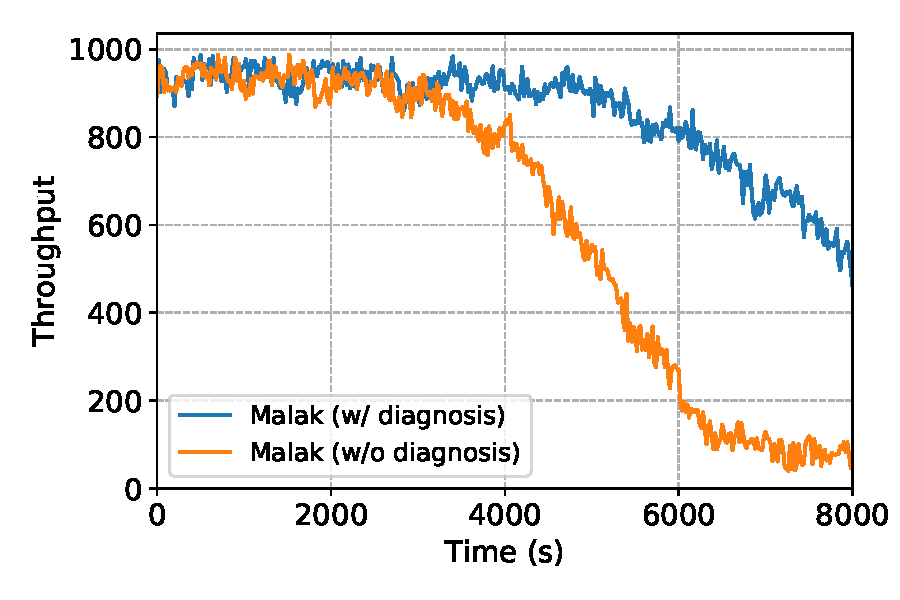
\includegraphics[width=.95\columnwidth]{Figure/diagnosis}
	\vspace{-0.1in}
	\caption{The performance improvement of automatic network repair.
		\textnormal{
			The automatic repair mechenism increases the average throughput by
			1.3 times compared with the basic {\sdn} routing algorithm, and
			2.2 and 3.9 times higher than RPL and LEACH, respectively.
		}}
	\label{fig:diagnosis}
\end{figure}

%\begin{figure}[htbp]
\begin{figure}[!h]
	\centering
	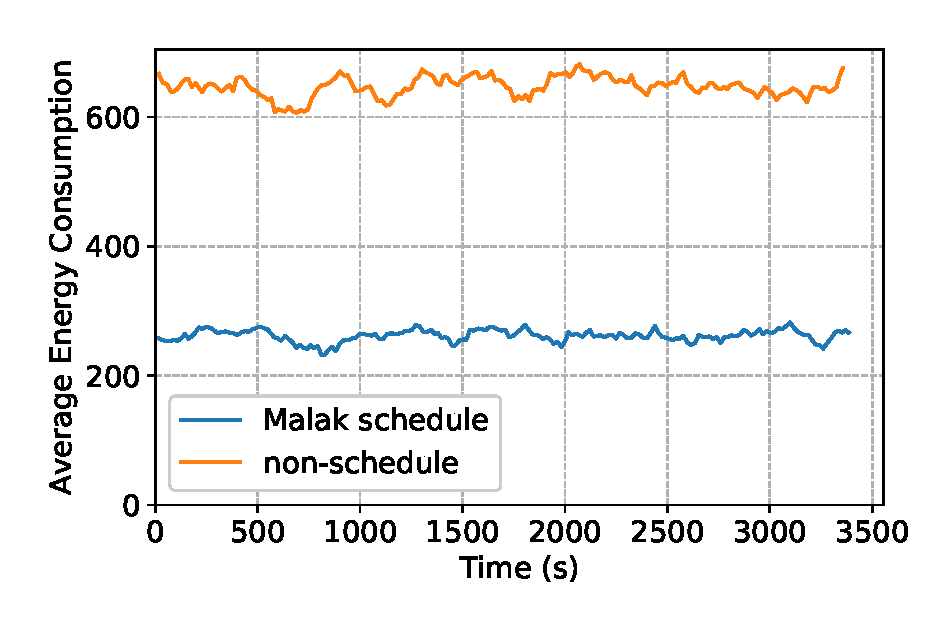
\includegraphics[width=.95\columnwidth]{Figure/multitask_energy}
	\vspace{-0.1in}
	\caption{Average energy consumption with and without multi-task schedule
		\textnormal{When with multi-task schedule, sensor consumes half of the energy
			comparing to when without multi-task schedule.}}
	\label{fig:multitask_energy}
\end{figure}

By applying multi-task schedule, we reduce the working sensors on one node and
the size of transmitted packets to cut down the energy consumption of sensing
and communication about 68.5\%.

